\begin{appendices}

\section{}
\label{appendix:replicone}

\begin{table}[h!] \centering 
  \caption{Replication results for one season for all dependent variables}
 % \label{appendix:replicone} 
\addtolength{\leftskip} {-2cm}
  \addtolength{\rightskip}{-2cm}
\begin{tabular}{@{\extracolsep{5pt}}lD{.}{.}{-3} D{.}{.}{-3} D{.}{.}{-3} D{.}{.}{-3} } 
\\[-1.8ex]\hline 
\hline \\[-1.8ex] 
\\ Difference H/A & \multicolumn{1}{c}{Goals} & \multicolumn{1}{c}{Points} & \multicolumn{1}{c}{Expected points} & \multicolumn{1}{c}{Shots} \\ 
\\[-1.8ex] & \multicolumn{1}{c}{(1)} & \multicolumn{1}{c}{(2)} & \multicolumn{1}{c}{(3)} & \multicolumn{1}{c}{(4)}\\ 
\hline \\[-1.8ex] 
 SpectatorsYes & 0.048 & 0.064 & 0.149^{***} & 1.333^{***} \\ 
  & (0.064) & (0.093) & (0.032) & (0.270) \\ 
  & & & & \\ 
 Constant & 0.226^{***} & 0.325^{***} & 0.284^{***} & 1.037^{***} \\ 
  & (0.054) & (0.082) & (0.028) & (0.231) \\ 
  & & & & \\ 
\hline \\[-1.8ex]
$\sigma^2_{u}$ & \multicolumn{1}{c}{0.00} & \multicolumn{1}{c}{0.00} & \multicolumn{1}{c}{0.00} & \multicolumn{1}{c}{0.00} \\ 
$\sigma^2_{e}$ & \multicolumn{1}{c}{2.99} & \multicolumn{1}{c}{6.42} & \multicolumn{1}{c}{0.74} & \multicolumn{1}{c}{53.49} \\ 
Observations & \multicolumn{1}{c}{3,752} & \multicolumn{1}{c}{3,752} & \multicolumn{1}{c}{3,752} & \multicolumn{1}{c}{3,752} \\ 
Log Likelihood & \multicolumn{1}{c}{-7,375.806} & \multicolumn{1}{c}{-8,812.464} & \multicolumn{1}{c}{-4,767.040} & \multicolumn{1}{c}{-12,789.320} \\ 
Akaike Inf. Crit. & \multicolumn{1}{c}{14,759.610} & \multicolumn{1}{c}{17,632.930} & \multicolumn{1}{c}{9,542.081} & \multicolumn{1}{c}{25,586.650} \\ 
Bayesian Inf. Crit. & \multicolumn{1}{c}{14,784.530} & \multicolumn{1}{c}{17,657.850} & \multicolumn{1}{c}{9,567.001} & \multicolumn{1}{c}{25,611.570} \\  
\hline 
\\Difference H/A & \multicolumn{1}{c}{Shots Target} & \multicolumn{1}{c}{Fouls} & \multicolumn{1}{c}{Yellow Cards} & \multicolumn{1}{c}{Red Cards} \\ 
\\[-1.8ex] & \multicolumn{1}{c}{(5)} & \multicolumn{1}{c}{(6)} & \multicolumn{1}{c}{(7)} & \multicolumn{1}{c}{(8)}\\ 
\hline \\[-1.8ex] 
 SpectatorsYes & 0.400^{**} & -0.745^{***} & -0.479^{***} & -0.034^{*} \\ 
  & (0.130) & (0.198) & (0.066) & (0.017) \\ 
  & & & & \\ 
 Constant & 0.418^{***} & 0.261 & 0.151^{**} & 0.002 \\ 
  & (0.111) & (0.179) & (0.056) & (0.014) \\ 
  & & & & \\ 
\hline \\[-1.8ex]
$\sigma^2_{u}$ & \multicolumn{1}{c}{0.00} & \multicolumn{1}{c}{0.03} & \multicolumn{1}{c}{0.00} & \multicolumn{1}{c}{0.00} \\ 
$\sigma^2_{e}$ & \multicolumn{1}{c}{12.43} & \multicolumn{1}{c}{28.73} & \multicolumn{1}{c}{3.17} & \multicolumn{1}{c}{0.21} \\ 
Observations & \multicolumn{1}{c}{3,752} & \multicolumn{1}{c}{3,752} & \multicolumn{1}{c}{3,752} & \multicolumn{1}{c}{3,752} \\ 
Log Likelihood & \multicolumn{1}{c}{-10,052.040} & \multicolumn{1}{c}{-11,625.370} & \multicolumn{1}{c}{-7,489.554} & \multicolumn{1}{c}{-2,408.555} \\ 
Akaike Inf. Crit. & \multicolumn{1}{c}{20,112.080} & \multicolumn{1}{c}{23,258.740} & \multicolumn{1}{c}{14,987.110} & \multicolumn{1}{c}{4,825.109} \\ 
Bayesian Inf. Crit. & \multicolumn{1}{c}{20,136.990} & \multicolumn{1}{c}{23,283.670} & \multicolumn{1}{c}{15,012.030} & \multicolumn{1}{c}{4,850.030} \\    
\hline 
\hline \\[-1.8ex] 
\textit{Note:}  & \multicolumn{4}{r}{$^{*}$p$<$0.05; $^{**}$p$<$0.01; $^{***}$p$<$0.001;} \\
& \multicolumn{4}{r}{$\sigma^2_{e}$ = Variance of first level residual error;}
& \multicolumn{5}{r}{$\sigma^2_{u}$ = Variance of second level residual error}
\end{tabular} 
\end{table} 

\newpage

\section{}
\label{appendix:replic}
\begin{figure}[H]
    \centering
    \caption{Replicated - Mean of all dependent variables for each season}
    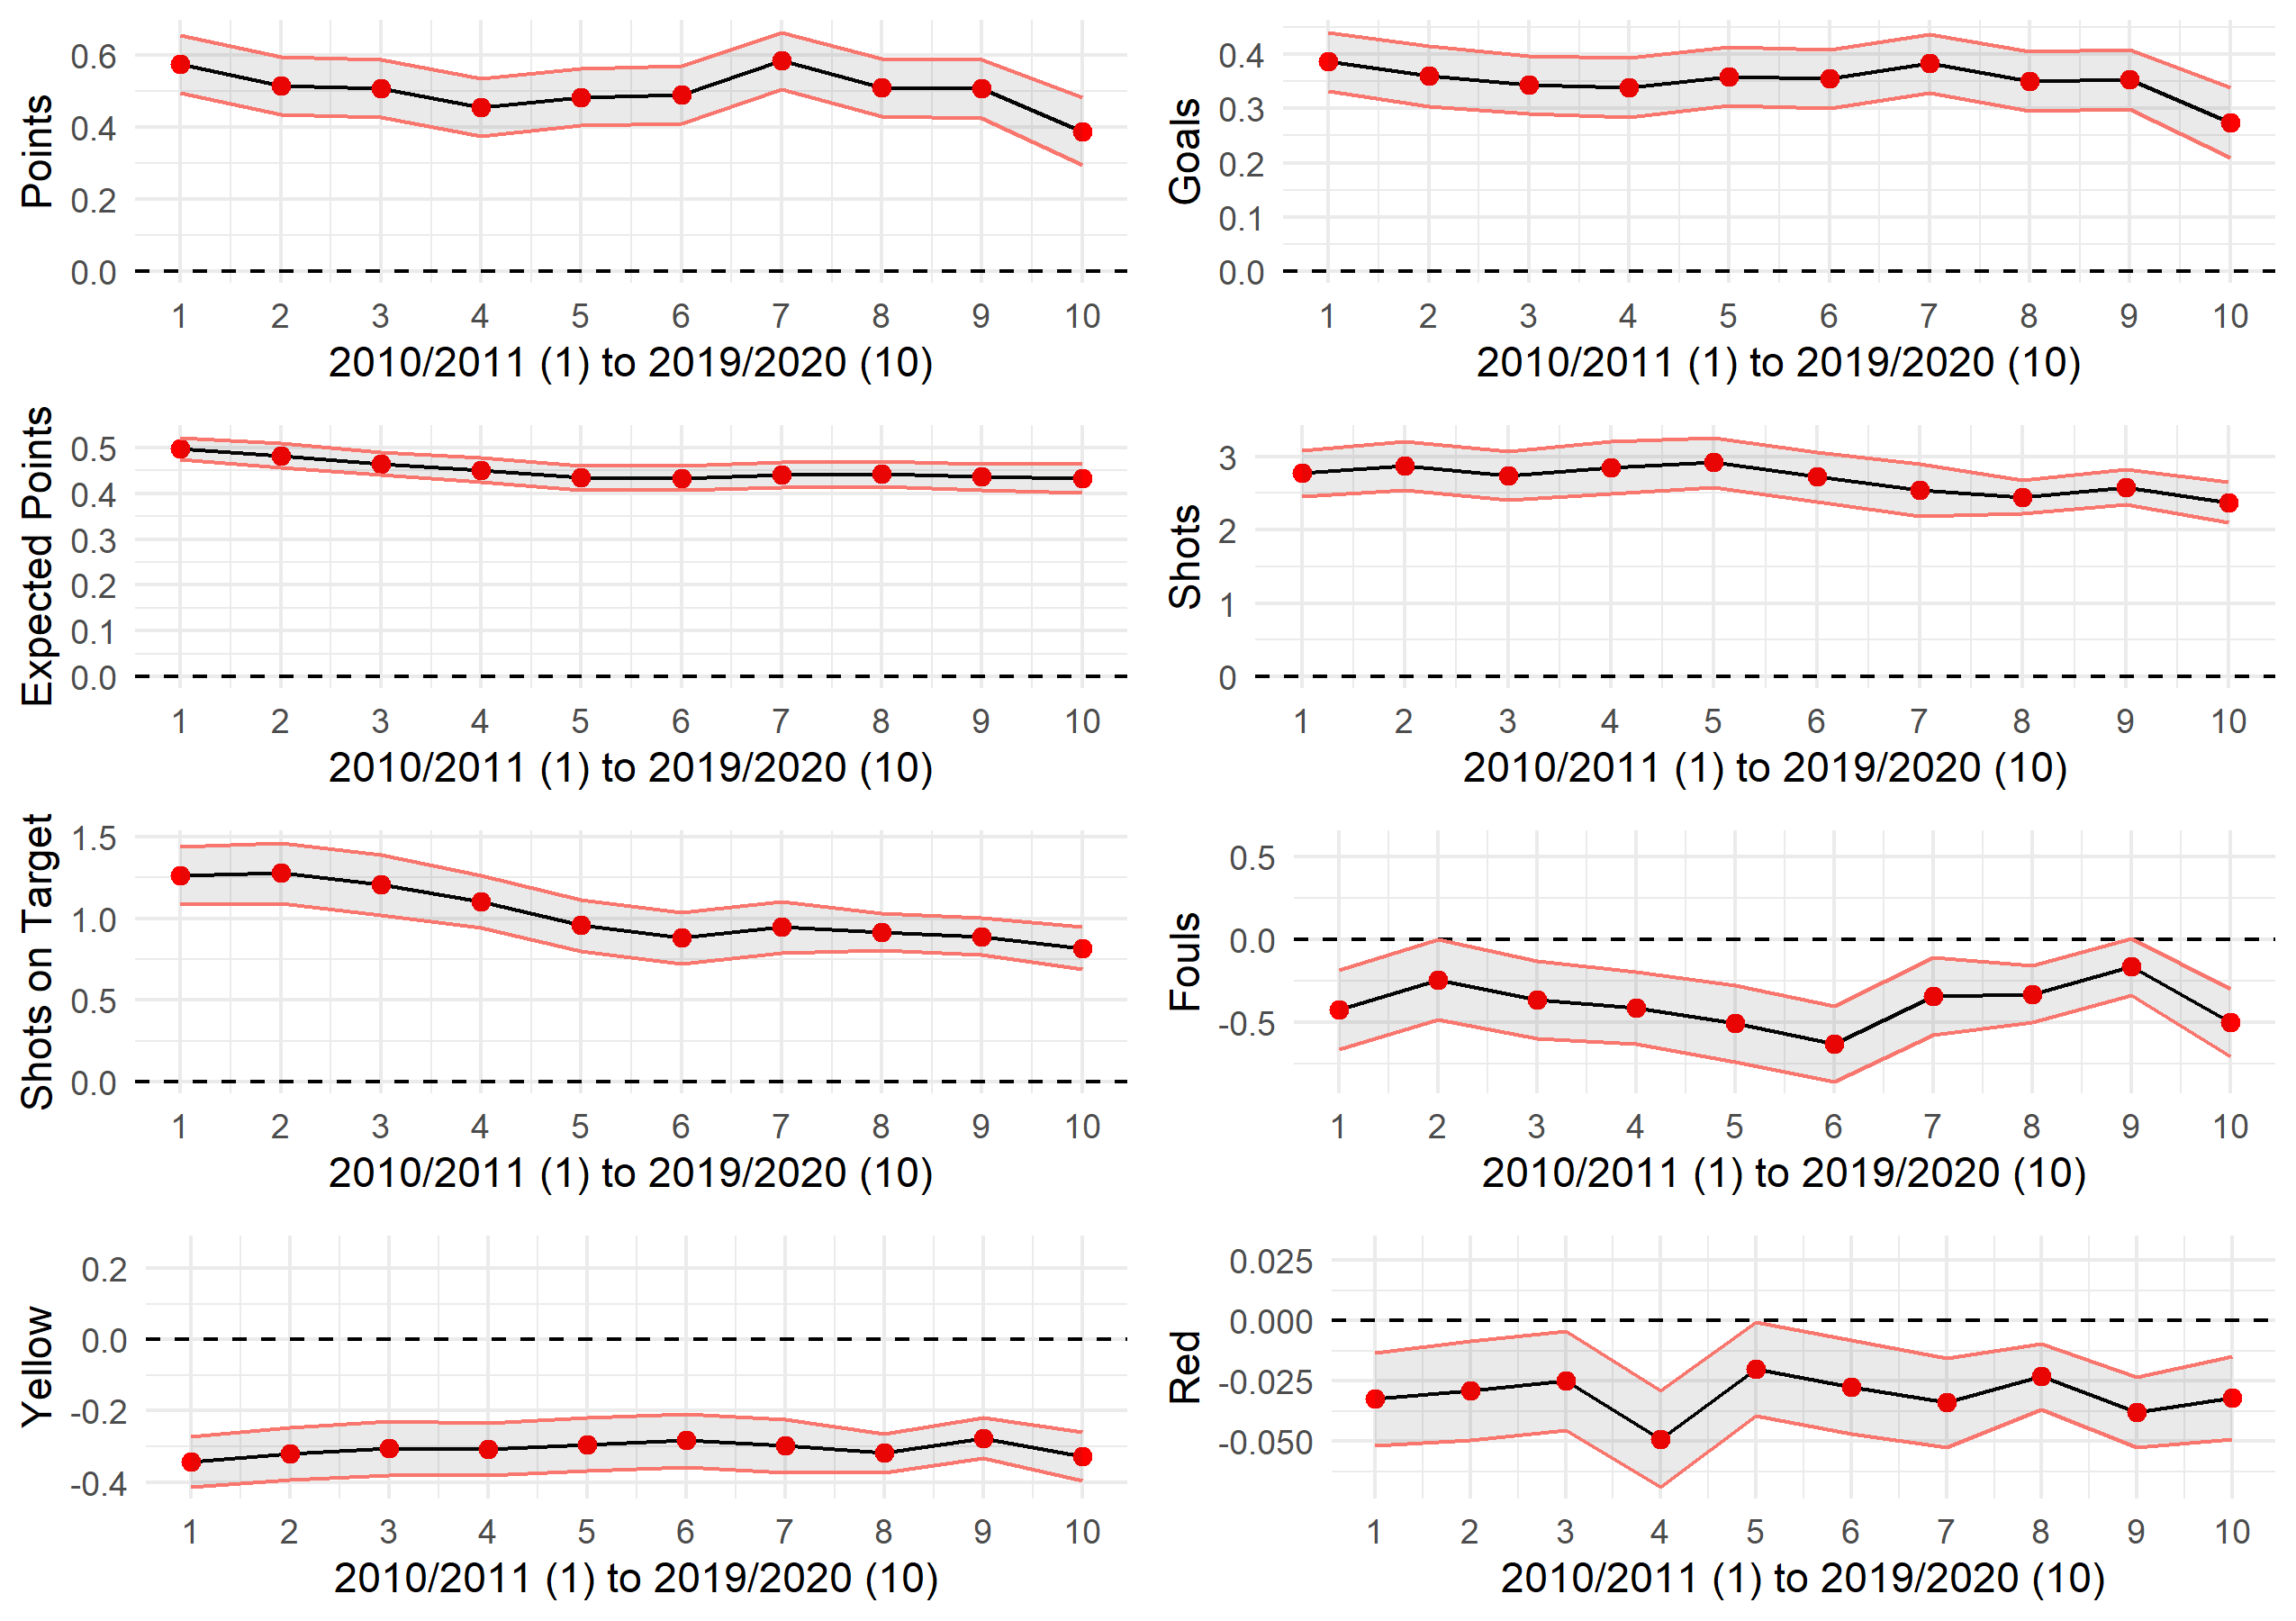
\includegraphics[width=1\textwidth]{Figures/Replicated_plot.png}
    %\label{appendix:replic}
\end{figure}
\newpage
\section{}
\label{appendix:explor}
\begin{figure}[H]
    \centering
    \caption{Exploratory - Mean of all dependent variables for each season}
    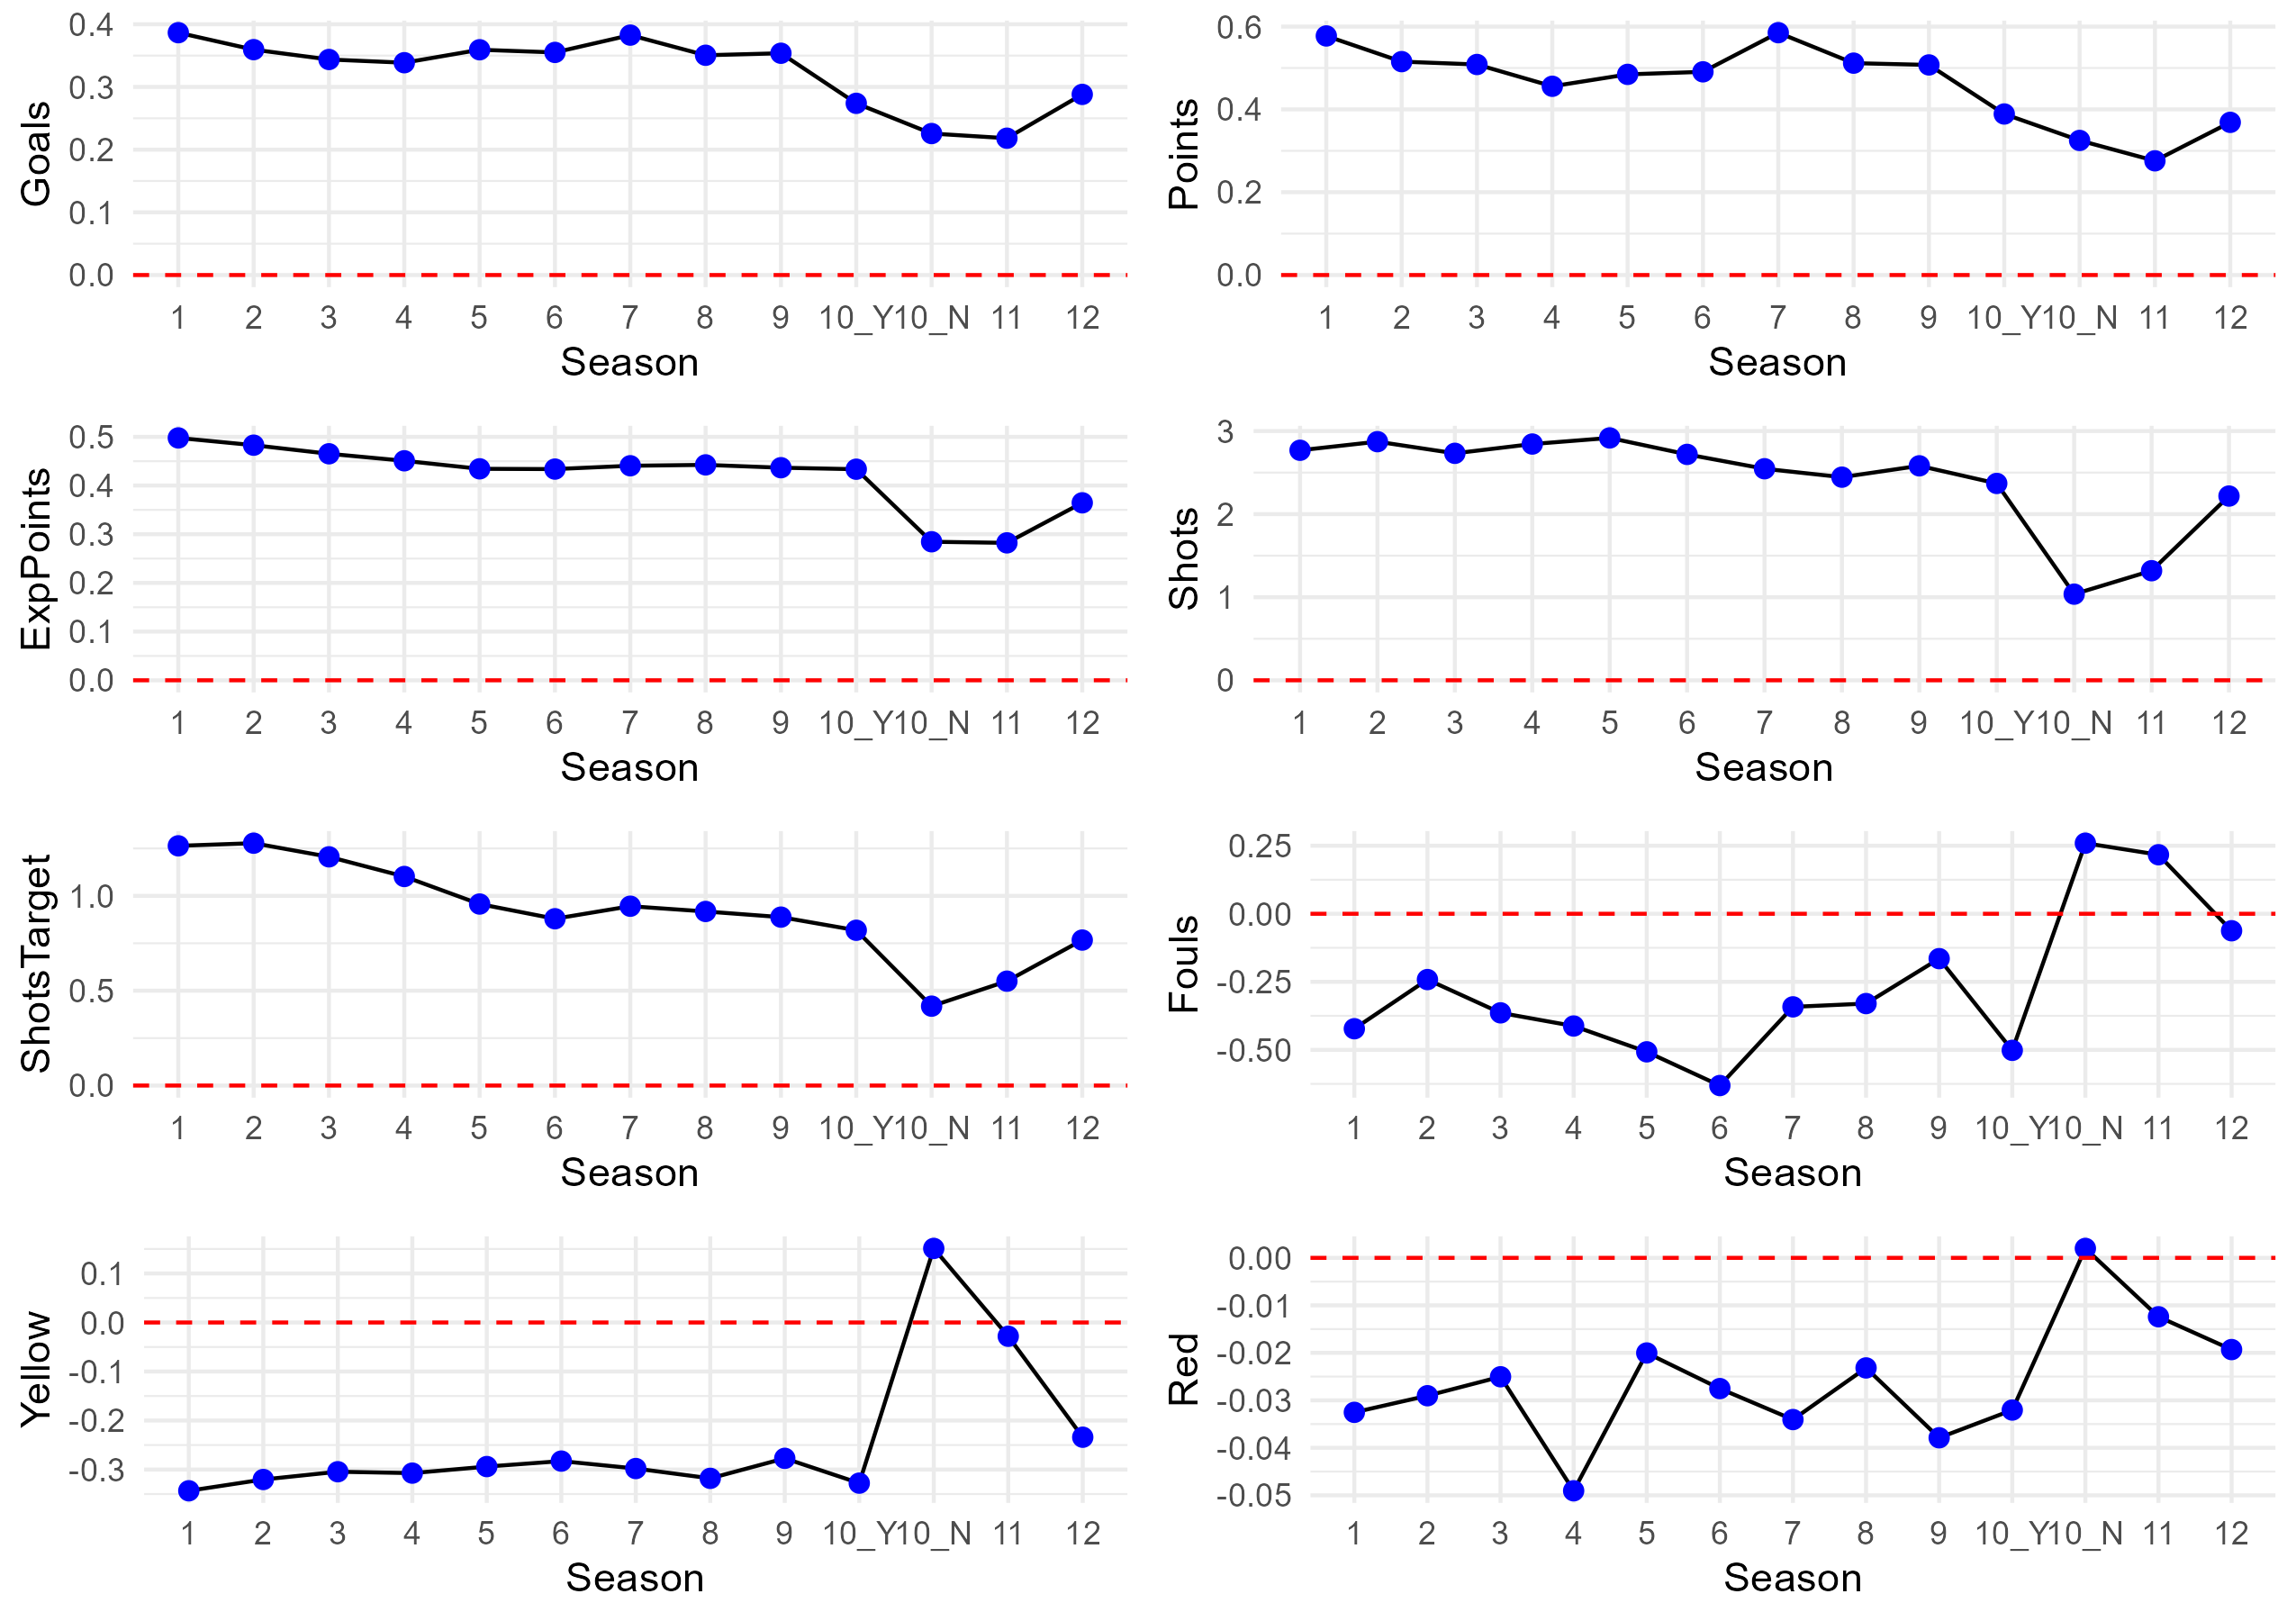
\includegraphics[width=1\textwidth]{Figures/Exploratory_plot.png}
    %\label{appendix:explor}
\end{figure}

\end{appendices}